\documentclass[12pt,letterpaper]{article}

%Note to Self:
%When Decommission? - after two months of feeling useless or right away?

\usepackage[utf8]{inputenc}
\usepackage[letterpaper,margin=1in]{geometry}
\usepackage{caption} % for table captions

\usepackage{amsmath} % for multi-line equations and piecewises
\usepackage{indentfirst} % to indent after a section
\usepackage{setspace}
\usepackage{times}
\usepackage{graphicx}
\usepackage{textcomp}
\usepackage{xspace}
\usepackage{verbatim} % for block comments
\usepackage{subfig} % for subfigures
\usepackage{enumitem} % for a) b) c) lists
\newcommand{\Cyclus}{\textsc{Cyclus}\xspace}%
\newcommand{\Cycamore}{\textsc{Cycamore}\xspace}%
\usepackage{tabularx}

\newcolumntype{b}{X}
\newcolumntype{s}{>{\hsize=.5\hsize}X}
\newcolumntype{m}{>{\hsize=.75\hsize}X}
\usepackage{titling}
\usepackage{minted}

\newcommand{\subtitle}[1]{%
  \posttitle{%
    \par\end{center}
    \begin{center}\large#1\end{center}
    \vskip0.5em}%
}
\usepackage{tikz}


\usetikzlibrary{shapes.geometric,arrows}
\tikzstyle{process} = [rectangle, rounded corners, minimum width=3cm, minimum height=1cm,text centered, draw=black, fill=blue!30]
\tikzstyle{arrow} = [thick,->,>=stealth]


\graphicspath{{images/}}
 
\usepackage[font={footnotesize,it}]{caption}
 



\setlength{\parindent}{15pt} % Default is 15pt.




\fontfamily{ptm}\selectfont

\title{Numerical Experiments for Verifying Demand Driven Deployment Algorithms}
\subtitle{Draft 2}
\author{Jin Whan Bae and Gwendolyn Chee}
\date{2017-10-11}


\begin{document}
	
	\maketitle
	\hrule
	\onehalfspacing
	\thispagestyle{empty}

\section{Introduction}
The Demand-Driven Cycamore Archetype project (NEUP-FY16-10512) aims to develop \Cycamore demand-driven deployment capabilities.
The project plans to use non-optimizing, deterministic-optimizing and stochastic-optimizing prediction algorithms.

These prediction models are being developed by the University of South Carolina. In this report, we discuss numerical experiments for testing the non-optimizing, deterministic optimizing and stochastic optimizing methods. The numerical experiments will be designed for both the once through nuclear fuel cycle and advanced fuel cycles. 

\section{Once through Nuclear Fuel Cycle}
\begin{figure}[H]
\caption{Flow Chart of Once through Nuclear Fuel Cycle}
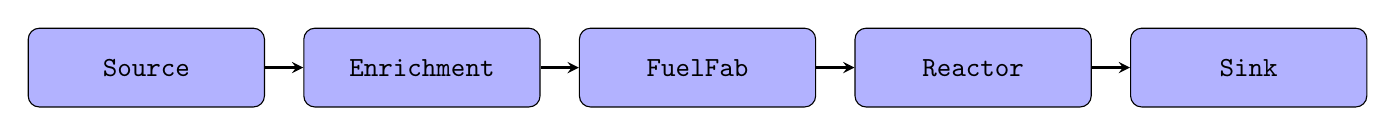
\begin{tikzpicture}[node distance=3.5cm]
\node (source) [process] {\texttt{Source}};
\node (enrichment) [process, right of=source] {\texttt{Enrichment}};
\node (fuelfab) [process, right of=enrichment] {\texttt{FuelFab}};
\node (reactor) [process, right of=fuelfab]{\texttt{Reactor}};
\node (sink) [process, right of=reactor]{\texttt{Sink}};

\draw [arrow] (source) -- (enrichment); 
\draw [arrow] (enrichment) -- (fuelfab); 
\draw [arrow] (fuelfab) -- (reactor);
\draw [arrow] (reactor) -- (sink);
\end{tikzpicture}
\end{figure}

In this report, the once-through fuel cycle is simplified to have 5 components: \texttt{Source}, \texttt{Enrichment}, \texttt{FuelFab}, \texttt{Reactor} and \texttt{Sink}. However, in a true once-through fuel cycle, there are more than 5 components. Other components include milling, conversion etc. For example, if a fuel cycle includes the milling step and excludes the \texttt{FuelFab} step, the tests can be modified to include milling and exclude \texttt{FuelFab}. 

\subsection{Input File Specification}
\Cyclus uses XML input files. For the input file, we assume the archetype to be an \texttt{INSTITUTION}, since it governs deployment and decommission of facilities.

The user would only have to define the reactor prototype and reactor deployment. 
The remaining fuel facilities,
both front end and back end, would be recognized by the archetype
by looking at each prototypes' in-and-out commodities.
Then the recognized, or `connected' fuel cycle facilities deploy
with demand.
If an input file does not have the necessary `connections' for the 
reactor to receive fuel, it will throw an error. 

We suggest an example format:
First, the input file would define reactor prototype to be deployed. There can be multiple reactors.

\begin{minted}{xml}
<institution>
      <name>NO_ddd</name>
       <config><NO_ddd/></config>
      <reactor_list>
        <val>lwr</val>
        <val>sfr</val>
        <val>mox_lwr</val>
      </reactor_list>
\end{minted}

Then deployment of the reactors is defined, and the user
is given the option to manually define the deployment(DeployInst):
\begin{minted}{xml}
      <deployment>
      <type>manual</type>

        <build_times>
          <val>1</val>
          <val>10</val>
          <val>20</val>
          <val>40</val>
        </build_times>
        <n_build>
          <val>3</val>
          <val>3</val>
          <val>3</val>
          <val>3</val>
        </n_build>
        <lifetimes>
          <val>960</val>
          <val>960</val>
          <val>960</val>
          <val>960</val>
        </lifetimes>
      </deployment>

    </institution>
\end{minted}

Or have the institution deploy reactors according to power demand (GrowthRegion):

\begin{minted}{xml}
      <deployment>
      <type>growth</type>

      <growth>
        <piecewise_function>
              <piece>
                <start>0</start>
                <function>
                  <type>linear</type>
                  <params>1 2</params>
                </function>
              </piece>
        </piecewise_function>
      </growth>
      
      </deployment>

    </institution>
\end{minted}

\subsection{Simple Scenario for Testing}

A simple scenario definition is given where a predefined \texttt{Reactor}
is deployed at timestep one and three. The chain of front---end
fuel cycle facility of one facility each 
(\texttt{Source}, \texttt{Enrichment}, \texttt{FuelFab}) can supply enough fuel
for the operation of one reactor. A \texttt{Sink} can hold enough
amount for two batches of fuel. The specifics are listed below:

\begin{table}[h]
     \centering
    \begin{tabularx}{\textwidth}{bbb}
       \hline
       Simulation Parameters & Value & Units \\
       \hline
       Duration & 7 & timesteps \\
       Deploy Reactors & 1, 3 & timesteps \\
       Natural U Composition & 0.71\% U235 & \\
       Tails Assay & 0.003 & \% U235 \\
       Fuel Enrichment & 4 & \% U235 \\
       Enrichment throughput & 300 & $\frac{kg}{month \cdot facility}$ \\
       Enrichment SWU Capacity & 2000 & $\frac{SWU}{month \cdot facility}$ \\
       Source Throughput & 3000 & $\frac{kg}{month \cdot facility}$\\
       Sink Capacity & 200 &  $\frac{kg}{facility}$ \\
       \hline
    \end{tabularx}
    \caption {Simulation Parameters}
    \label{tab:reactor}
\end{table}

\begin{table}[h]
    \centering
    \begin{tabularx}{\textwidth}{bbb}
       \hline
       Reactor Parameters & Value & Units \\
       \hline
       Cycle Time & 2 & timesteps \\
       Refuel Time & 1 & timesteps \\
       Lifetime & 6 & timesteps \\
       Power Capacity & 1000 & MWe \\
       Assembly Size & 100 & kg \\
       \# assemblies per core & 3 & \\
       \# assemblies per batch & 1 & \\
       \hline
    \end{tabularx}
    \caption {Reactor Parameters}
    \label{tab:reactor}
\end{table}


An example input file with the facility and simulation
definitions can be found in the input directory of this repository.

\newpage
\subsection{Analytical Solution}
The simple scenario is solve analytically.

\begin{table}[h]
    \centering
    \begin{tabularx}{\textwidth}{ssmmmb}
       \hline
       Timestep & Fuel [kg] & Enrichment [$\frac{SWU}{month}$]& Source [$\frac{kg}{month}$] & Sink Capacity [kg] & Note\\
       \hline
       1 & 300 & 1583 & 2701 & 0 & Reactor1 core load\\
       2 & 0 & 1583 & 2701 & 0 & \\
       3 & 400 & 2111 & 3601 & 100 & Reactor2 core load, Reactor1 refuel\\
       4 & 0 & 2111 & 3601 & 0 & \\
       5 & 100 & 528 & 901 & 200 & Reactor2 refuel\\
       6 & 0 & 528 & 901 & 500 & Reactor1 decom \\
       7 & 0 & 528 & 901 & 500 & \\
       8 & 0 & 528 & 901 & 800 & Reactor2 decom\\
       9 & 0 & 528 & 901 & 800 & \\
       \hline
    \end{tabularx}
    \caption {Analytical Solution}
    \label{tab:analytical}
\end{table}


\begin{table}[H]
    \centering
    \begin{tabularx}{\textwidth}{ssss}
       \hline
       & Deploy & Deploy & Deploy \\
       Timestep & Enrichment & Source & Sink  \\
       \hline
       1 & \textcolor{red}{1} & \textcolor{red}{1} & 0  \\
       2 & 0 & 0 & 0  \\
       3 & \textcolor{red}{1} & 0 & \textcolor{red}{1}  \\
       4 & 0 & \textcolor{red}{1} & 0  \\
       5 & 0 & 0 & 0  \\
       6 & 0 & 0 & \textcolor{red}{2}  \\
       7 & 0 & 0 & 0  \\
       8 & 0 & 0 & \textcolor{red}{1}  \\
       9 & 0 & 0 & 0  \\
       \hline
    \end{tabularx}
    \caption {Deployment Needs}
    \label{tab:deployment}
\end{table}




\subsection{Non-optimizing prediction method}
The following conditions need to be satisfied for each segment of the fuel cycle. 

\subsubsection{\texttt{Reactor}}

\begin{enumerate}
 
\item Do all the \texttt{Reactor}s run? 
\item  Do all the \texttt{Reactor}s run at full capacity (not lacking fuel)? 

\item Is a new \texttt{Reactor} deployed when the energy demand exceeds the energy produced by the current \texttt{Reactor}s? 

\item Is a \texttt{Reactor} decommissioned when the energy demand falls behind the output of the current \texttt{Reactor}s? 

\end{enumerate}

\subsubsection{\texttt{Fuelfab}}
\begin{enumerate}
\item  Is the fuel produced by the \texttt{Fuelfab} within the upper limit of [insert uncertainty] for the analytic solution of fuel required by the \texttt{Reactor}s for all of them to run for each time step? 

\item Is a new \texttt{Fuelfab} deployed when the fuel required by the reactors exceeds the output of current \texttt{Fuelfab}?

\item Is a \texttt{Fuelfab} decommissioned when the fuel required by the reactors falls behind the output of current \texttt{Fuelfab} facilities?
\end{enumerate}

\subsubsection{\texttt{Enrichment}}
\begin{enumerate}
\item  Is the enriched uranium produced by \texttt{Enrichment} within the upper limit of [insert uncertainty] for the analytic solution of the enriched uranium required by the \texttt{Fuelfab} for each time step? 

\item Is a new \texttt{Enrichment} facility deployed when the enriched uranium required by the \texttt{Fuelfab} exceeds the enriched uranium produced of current \texttt{Enrichment} facilities?

\item Is a \texttt{Enrichment} decommissioned when the enriched uranium required by the \texttt{Fuelfab} falls behind the enriched uranium produced by current \texttt{Enrichment} facilities?
\end{enumerate}

\subsubsection{\texttt{Source}}
\begin{enumerate}
\item Is the mined uranium produced by \texttt{Source} within the upper limit of [insert uncertainty] for the analytic solution of the mined uranium required by the \texttt{Enrichment} facilities for each time step? 

\item Does the \texttt{Source} mined uranium produced increase when mined uranium required by the \texttt{Enrichment} facilities exceeds mined uranium produced by the current \texttt{Source}?

\item Does the \texttt{Source} mined uranium produced decrease when mined uranium required by the \texttt{Enrichment} facilities falls behind the mined uranium required by the current \texttt{Source}?
\end{enumerate}

\subsection{Deterministic-Optimizing/Stochastic prediction method}
The following conditions need to be satisfied for each segment of the fuel cycle. 

\begin{enumerate}
\item Do all the \texttt{Reactor}s run? 
\begin{minted}{c++}
TEST(ReactorTests, DDDeploy_DO) {
    [Example input with the following attributes:]
        [int simdur = 20;]
        [Defines reactor with zero refueling cycle and operation 
        cycle of 1 month]
        [Defines fuel cycle facilities parameters]
        [Defines Reactor Deploy Scheme / Power Demand]
        [Increasing Fuel Demand with Time]
    [Run test]
    [Test if Reactor has no zero values in output Timeseriespower]
}
\end{minted}
\item  Do all the \texttt{Reactor}s run at full capacity (not lacking fuel)? 
\begin{minted}{c++}
TEST(ReactorTests, DDDeploy_DO) {
    [Example input with the following attributes:]
        [int simdur = 20;]
        [Defines reactor with zero refueling cycle, power capacity 
        of x and operation cycle of 1 month]
        [Defines fuel cycle facilities parameters]
        [Defines Reactor Deploy Scheme / Power Demand]
        [Increasing Fuel Demand with Time]
    [Run test]
    [Test if Reactor has x value in output Timeseriespower]
}
\end{minted}

\item Is the objective function optimized?

\item Is the constraint followed? 

\item  Do the related fuel cycle facilities get deployed upon demand?
\begin{minted}{xml}
TEST(ReactorTests, DDDeploy_NO) {
    [Example input with the following attributes:]
        [int simdur = 20;]
        [Defines reactor with zero refueling cycle and operation 
        cycle of 1 month]
        [Defines fuel cycle facilities parameters]
        [Defines Reactor Deploy Scheme / Power Demand]
        [Increasing Fuel Demand with Time]
    [Run test]
    [Test if fuel facility is deployed in the beginning]
    [Test if fuel facility is deployed later in the simulation 
    (have analytic solution)]
}
\end{minted}

\item Do the related fuel cycle facilities exit upon demand decrease?
\begin{minted}{xml}
TEST(ReactorTests, DDDeploy_NO) {
    [Example input with the following attributes:]
        [int simdur = 20;]
        [Defines reactor with zero refueling cycle and operation 
        cycle of 1 month]
        [Defines fuel cycle facilities parameters]
        [Defines Reactor Deploy Scheme / Power Demand]
        [Decreasing Fuel Demand with Time]
    [Run test]
    [Test if fuel facility is deployed in the beginning]
    [Test if fuel facility exits later in the simulation (have 
    analytic solution)]
}
\end{minted}


\end{enumerate}





\section{Advanced Fuel Cycles}
\end{document}






